\section{Notifications Module}

\subsection{Overview}
The Notification Module is a core module that is responsible for delivering  messages to system users via said users' preferred method of communication. Messages might include add on system updates that a user indicated they want to receive, or any other system related updates. Notifications will be sent via a medium external to the application, using ether SMS or email services. The Notification Module shall be implemented in such a way that it can handle messages concurrently, and clients requesting the service shall not be blocked until the request has executed.

\subsection{Use Cases}
\paragraph{Send and Receive}
Registered users will be able to receive notifications such as system updates and add on specific notifications. Admin users will be able to broadcast notifications, and add on systems will be able to notify users of their specific updates. To transmit a message, the request must first be validated. Validation includes request and system integrity checks, and validation of sending users. Only users that have admin rights can send messages. If an add on subsystem requires the service, it must first allocate a proxy admin user dedicated to said add on system.

\begin{figure}[H]
\centering
\includegraphics[width=0.8\linewidth]{\imgPath/notifications-use-case}
\caption{Notifications Request and Send Use Case}
\end{figure}

\paragraph{Notification Profile}
Registered users will be able to chose their means of communication and customize their notification profile.
\begin{figure}[H]
\centering
\includegraphics[width=1\linewidth]{\imgPath/notifications-profile-use-case}
\caption{Notifications Profile Use Case}
\end{figure}

\subsection{Classes}
The Notification Module will be comprised of a manager class i.e. NotificationManager, a request class i.e. NotificationRequest, a class related to the users' profile, i.e. NotificationProfile, and a class that will handle sending of the notification i.e. NotificationSender.

\paragraph{NotificationManager}
NotificationManager will maintain and store user profiles related to notifications, validate requests, and invoke the apropriate transmission service.

\paragraph{NotificationRequest}
NotificationRequest is a abstract class that will contain the message to transmit, the serialization thereof, and the target user. An optional runnable callback object can be attached that will be invoked in the event of failure of any kind. this will allow the operation of sending a request to be non-blocking, while providing a means of error tracing and correcting.

\paragraph{NotificationProfile}
NotificationProfile will store system uses' preferred means of communication, i.e. SMS and/or email.

\paragraph{NotificationSender}
NotificationSender will implement the relevant technical requirements to use the underling service type, e.g. SMS service. A modular system is used that will simplify addition of additional transmission services. If such service is complex, a bridge pattern can be implemented with little difficulty.

\subsection{Design Patterns}
Singleton, Command, and Strategy design patterns must be used to implement the Notification Module.

\paragraph{Singleton}
The Singleton pattern will provide a well known entry point to access and make use of the service. This is well suited, as only one manager class for the Notification Module must be instantiated. 

\paragraph{Command}
A modified version of the Command pattern must be implemented, where systems requesting to send a notification must implement there own concrete NotificationRequest class. The abstract method to be implemented is the serialization of the request object. This will decouple the systems that intend to send notifications from the Notification Module, and allow flexibility to implement add on specific notifications.

\paragraph{Strategy}
Two methods to transmit the notification must be implemented i.e. emails and SMS. The appropriate method (i.e. the method dictated by the user's profile) must be used to convey the notification. The Strategy pattern will allow the profile specific method to be used when transmitting the notification, while providing the implementation that is dependent on the underlying transmission system.

\begin{figure}[H]
\centering
\includegraphics[width=1.2\linewidth]{\imgPath/notification-class-diagram}
\caption{Notifications Class Diagram}
\end{figure}

\begin{figure}[H]
\centering
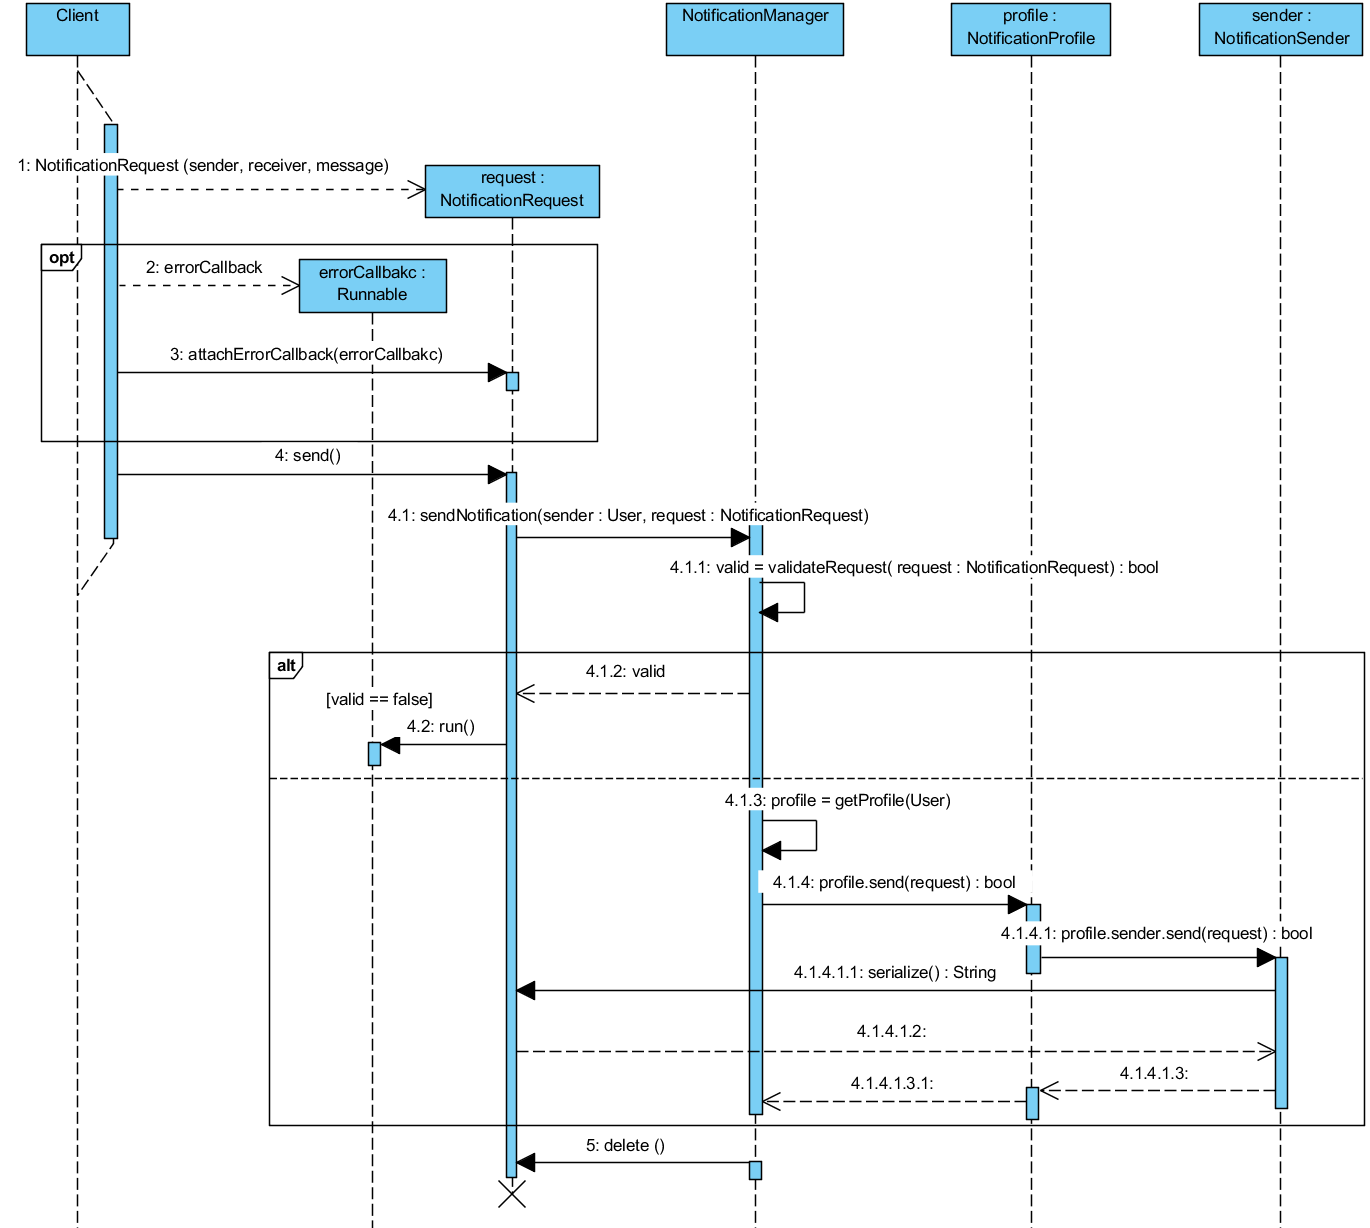
\includegraphics[width=1.2\linewidth]{\imgPath/notification-module-client-interaction}
\caption{Notification Module - Client Interaction}
\end{figure}

\begin{figure}[H]
\centering
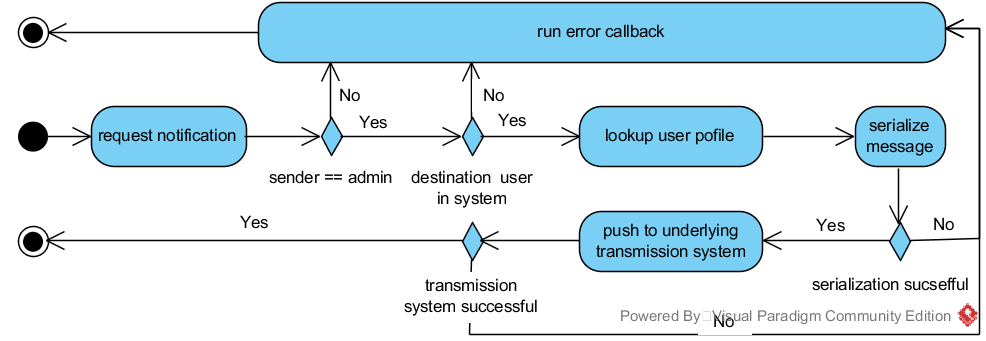
\includegraphics[width=1.0\linewidth]{\imgPath/notification-activity-send}
\caption{Notification Module - Request Notification}
\end{figure}


\subsection{Technologies}

\paragraph{Email}
Authenticated SMTP must be used to send messages to the email server that NavUp will use. This is to prevent the email server from relaying messages that are not properly validated. Internet Message Access Protocol (IMAP) will be used to store emails, as this is most prevalent system and thus support aught to be sufficient. POP3 might be an option as emails need not be stored for extended periods after the email has been delivered. TCP/IP will be used implicitly.

\paragraph{SMS}
A Direct-to-SMS gateway will be the most appropriate service to use, encoding all messages in plain ASCII text to promote device compatibility. The infrastructure such as GSM is determined by the service provider.